%% sicp.tex
%% Mac Radigan
%
%% SICP documentation

\documentclass{article}[11pt]
\usepackage[]{graphics}
%\usepackage{titlesec}

%\usepackage[framed,numbered,autolinebreaks,useliterate]{mcode}
\usepackage{setspace}
\usepackage[left=1in,top=1in,right=1in,bottom=1in,nohead]{geometry}
\usepackage{graphicx,amssymb,amstext,amsmath,amsthm,caption,mathtools}
\usepackage{algorithm}
\usepackage{algorithmic}
\usepackage{amsfonts}
\usepackage{amssymb}
\bibliographystyle{IEEEtran}
%\usepackage{csvtools}
\usepackage{pdftexcmds}
%\usepackage{minted}
\usepackage{fancyvrb}
\usepackage{float}
\usepackage{csquotes}
\usepackage[skins,minted]{tcolorbox}
%\titleformat{\section}[block]{\Large\bfseries\filcenter}{}{}{}
%\newcommand\Quote[1]{\lq\textsl{#1}\rq}
%\newcommand\fr[2]{{\textstyle\frac{#1}{#2}}}
%\newcommand{\ssection}[1]{\section[#1]{\centering\normalfont\scshape #1}}
%\newcommand{\ssubsection}[1]{\subsection[#1]{\raggedright\normalfont\itshape #1}}

\usepackage{mdframed}

\usepackage{hyperref}
\hypersetup{
  colorlinks,
  citecolor=black,
  filecolor=black,
  linkcolor=black,
  urlcolor=black
}

\definecolor{bashbg}{rgb}{0.95,0.95,0.95}
\definecolor{schemebg}{rgb}{0.95,0.95,0.95}
\definecolor{outbg}{rgb}{0.98, 0.98, 0.82}

\newcommand{\bashlist}[1]{
 \begin{mdframed}[linecolor=black, topline=true, bottomline=true, leftline=false, rightline=false, backgroundcolor=bashbg]
 \inputminted[
   fontfamily=tt,
   fontsize=\footnotesize,
   linenos=true,
   numberblanklines=true,
   numbersep=12pt,
   numbersep=5pt,
   frame=leftline,
   breaklines=true
 ]{bash}{#1}
 \end{mdframed}
}

\newcommand{\schemelist}[1]{
 \begin{mdframed}[linecolor=black, topline=true, bottomline=true, leftline=false, rightline=false, backgroundcolor=schemebg]
 \inputminted[
   fontfamily=tt,
   fontsize=\footnotesize,
   linenos=true,
   numberblanklines=true,
   numbersep=12pt,
   numbersep=5pt,
   frame=leftline,
   breaklines=true
 ]{scheme}{#1}
 \end{mdframed}
}

\newcommand{\schemelistOLD}[1]{
 \inputminted[
   bgcolor=schemebg,
   fontfamily=tt,
   linenos=true,
   numberblanklines=true,
   numbersep=12pt,
   numbersep=5pt,
   gobble=0,
   frame=leftline,
   framesep=2mm,
   funcnamehighlighting=true,
   tabsize=4,
   obeytabs=false,
   mathescape=false
   samepage=false,
   showspaces=false,
   showtabs =false,
   texcl=false,
   baselinestretch=1.2,
   fontsize=\footnotesize,
   breaklines=true
 ]{scheme}{#1}
}

\newcommand{\outlist}[1]{
 \inputminted[
   bgcolor=outbg,
   fontfamily=tt,
   linenos=false,
   numberblanklines=false,
   numbersep=12pt,
   numbersep=5pt,
   gobble=0,
   frame=leftline,
   framesep=2mm,
   funcnamehighlighting=true,
   tabsize=4,
   obeytabs=false,
   mathescape=false
   samepage=false,
   showspaces=false,
   showtabs =false,
   texcl=false,
   baselinestretch=1.2,
   fontsize=\footnotesize,
   breaklines=true]{scheme}{#1}
}

\begin{document}

\title{Structure and Interpretation of Computer Programs (SICP) \\ worked examples}
\author{Mac Radigan}
\date{} % comment this out if you would like to include the date
\doublespacing

\maketitle

\begin{abstract}
A collection of worked examples from Gerald Sussman's book Structure and Interpretation of Computer Programs (SICP) \cite{sicp}.
\end{abstract}

\tableofcontents
%\listoffigures

%% Chapter-1.tex
%% Mac Radigan
%
%% Examples from SICP Chapter 1

    \section{Building Abstractions with Procedures}
        \subsection{The Elements of Programming}
            \subsubsection{Expressions}
              \schemelist{../chapter-1/sicp_ch1_e1-1.scm}
              \outlist{../output/sicp_ch1_e1-1.out}
            \subsubsection{Naming and the Environment}
              \schemelist{../chapter-1/sicp_ch1_e1-2.scm}
              \outlist{../output/sicp_ch1_e1-2.out}
            \subsubsection{Evaluating Combinations}
              \schemelist{../chapter-1/sicp_ch1_e1-3.scm}
              \outlist{../output/sicp_ch1_e1-3.out}
            \subsubsection{Compound Procedures}
              \schemelist{../chapter-1/sicp_ch1_e1-4.scm}
              \outlist{../output/sicp_ch1_e1-4.out}
            \subsubsection{The Substitution Model for Procedure Application}
              % infinite loop (do not include output listing)
              \schemelist{../chapter-1/sicp_ch1_e1-5.scm}
              \outlist{../output/sicp_ch1_e1-5.out}
            \subsubsection{Conditional Expressions and Predicates}
            \subsubsection{Example: Square Roots by Newton's Method}
              \schemelist{../chapter-1/sicp_ch1_e1-7.scm}
              \outlist{../output/sicp_ch1_e1-7.out}
            \subsubsection{Procedures as Black-Box Abstractions}
        \subsection{Procedures and the Processes They Generate}
            \subsubsection{Linear Recursion and Iteration}
              \schemelist{../chapter-1/sicp_ch1_e1-9.scm}
              \outlist{../output/sicp_ch1_e1-9.out}

Representing State Space Transitions
\newline

\begin{displayquote}
There are only two hard things in Computer Science: cache invalidation and naming things.
\newline
- Phil Karlton
\end{displayquote}

Recursive Definition
\newline

\begin{equation}
f\left(n\right) = 
\begin{cases}
n & n < 3 \\
1 f\left(n-1\right) + 2 f\left(n-2\right) + 3 f\left(n-3\right) & \mbox{ otherwise }
\end{cases}
\label{eq:ss_recursive}
\end{equation}

Direct Iterative Implementation
\newline

\begin{equation}
f\left(n\right) \coloneqq s_0
\label{eq:direct_def}
\end{equation}

with state transition

\begin{equation}
\stackrel{\mbox{T}}{
\left[ \begin{array}{c}
s_0 \leftarrow s_0 + 2 s_1 + 3 s_2 \\
s_1 \leftarrow s_0 \\
s_2 \leftarrow s_1 \\
\end{array} \right]
}
\label{eq:direct_trans}
\end{equation}

and initial conditions

\begin{equation}
\stackrel{\mbox{$S_0$}}{
\left[ \begin{array}{c}
s_0 \coloneqq 2 \\
s_1 \coloneqq 1 \\
s_2 \coloneqq 0 \\
\end{array} \right]
}
\label{eq:direct_init}
\end{equation}

Linear Feedback Shift Register (LFSR) representation
\newline

\begin{equation}
f\left(n,\underbar{s}\right)
\leftarrow
\begin{cases}
n^{th}_1 \underbar{s} & n = 0 \\
f\left( n-1, n^{th}_1 \leftangle \sigma_{1}(\underbar{s}), \left[ 1,2,3 \right] \rightangle \right) & \mbox{ otherwise }
\end{cases}
\label{eq:lfsr_def}
\end{equation}

\begin{equation}
\leftangle x, y \rightangle
\triangleq
\sum_{k} x_k y_k 
= x_k y^k
\label{eq:dotprod}
\end{equation}

\begin{equation}
n^{th}_k
\triangleq
x_k
\label{eq:nth}
\end{equation}

\begin{equation}
\sigma_k \left( \underbar{x} \right)
\triangleq
x_{\left( n + k \right) mod |x|} \forall n \in \underbar{x}
\label{eq:rotate}
\end{equation}

\begin{figure}[H]
\begin{center}
%\resizebox{7in}{!}{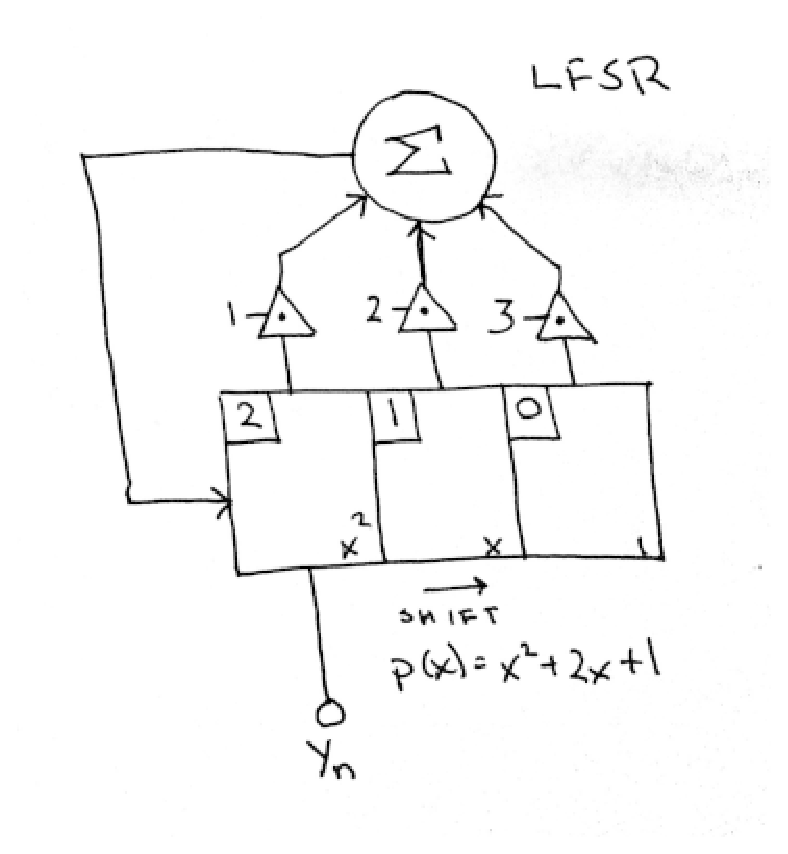
\includegraphics{./figures/lfsr-2.eps}
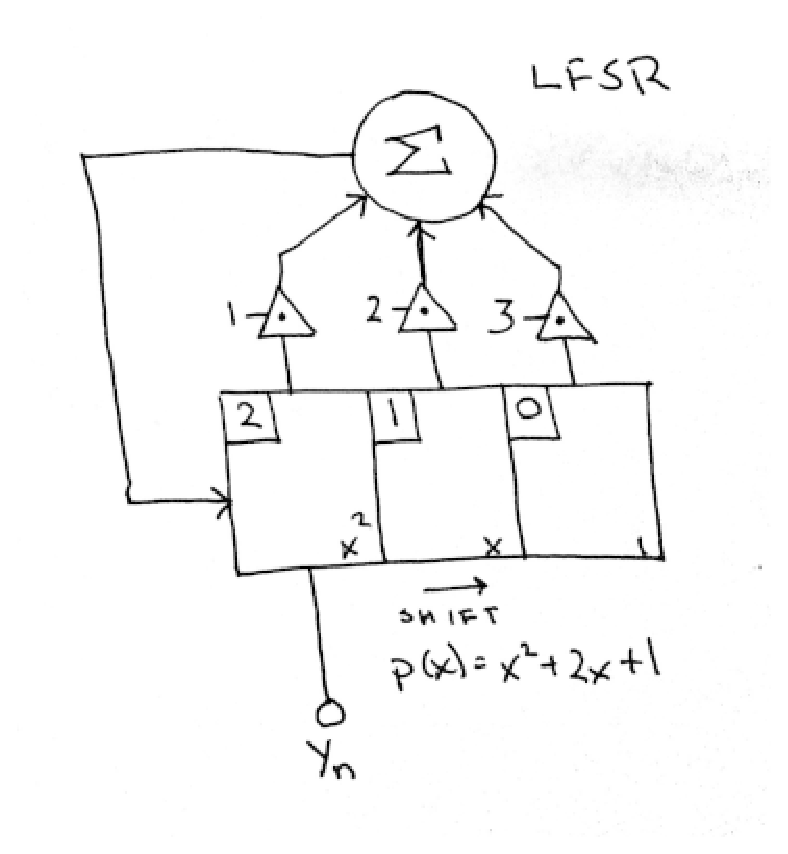
\includegraphics{./figures/lfsr-2.eps}
\end{center}
\caption{Linear Feedback Shift Register (LFSR)}
\label{fig:lfsr}
\end{figure}

State Space Representation
\newline

\begin{equation}
\mathbf{X}_k = \mathbf{F}\mathbf{X}_{k-1}
\label{eq:ss_rep}
\end{equation}

\begin{equation}
\stackrel{\mbox{$X_k$}}{
\left[ \begin{array}{c}
x^{'}_{0} \\
x^{'}_{1} \\
x^{'}_{2} \\
\end{array} \right]
}
= 
\stackrel{\mbox{$F$}}{
\left[ \begin{array}{ccc}
1 & 2 & 3 \\
1 & 0 & 0 \\
0 & 1 & 0 \\
\end{array} \right]
}
\stackrel{\mbox{$X_{k-1}$}}{
\left[ \begin{array}{c}
x_{0} \\
x_{1} \\
x_{2} \\
\end{array} \right]
}
\label{eq:ss_rep_2}
\end{equation}

where

\begin{equation}
\mathbf{X}_0 = 
\stackrel{\mbox{$X_{0}$}}{
\left[ \begin{array}{c}
2 \\
1 \\
0 \\
\end{array} \right]
}
\label{eq:ss_x0}
\end{equation}

so

\begin{equation}
\mathbf{X}_k 
= \mathbf{F}\mathbf{X}_{k-1}
= \mathbf{F} \left( \mathbf{F}\mathbf{X}_{k-2} \right)
= \mathbf{F} \left( \mathbf{F} \left( \mathbf{F}\mathbf{X}_{k-3} \right) \right)
= \cdots
= \mathbf{F}^N \mathbf{X}_0
\label{eq:ss_rep_expanded}
\end{equation}

              \schemelist{../chapter-1/sicp_ch1_e1-11.scm}
              \outlist{../output/sicp_ch1_e1-11.out}
            \subsubsection{Tree Recursion}
            \subsubsection{Orders of Growth}
            \subsubsection{Exponentiation}
              \schemelist{../chapter-1/sicp_ch1_e1-16.scm}
              \outlist{../output/sicp_ch1_e1-16.out}
            \subsubsection{Greatest Common Divisors}
            \subsubsection{Example: Testing for Primality}
        \subsection{Formulating Abstractions with Higher-Order Procedures}
            \subsubsection{Procedures as Arguments}
            \subsubsection{Constructing Procedures Using Lambda}
            \subsubsection{Procedures as General Methods}
            \subsubsection{Procedures as Returned Values}
              \schemelist{../chapter-1/sicp_ch1_e1-42.scm}
              \outlist{../output/sicp_ch1_e1-42.out}

%% *EOF*

%% Chapter-1.tex
%% Mac Radigan
%
%% Examples from SICP Chapter 2

    \section{Building Abstractions with Data}
        \subsection{Introduction to Data Abstraction}
            \subsubsection{Example: Arithmetic Operations for Rational Numbers}
              \schemelist{../chapter-2/sicp_ch2_e1-1.scm}
              \outlist{../output/sicp_ch2_e1-1.out}
            \subsubsection{Abstraction Barriers}
              \schemelist{../chapter-2/sicp_ch2_e1-2.scm}
              \outlist{../output/sicp_ch2_e1-2.out}
              \schemelist{../chapter-2/sicp_ch2_e1-3.scm}
              \outlist{../output/sicp_ch2_e1-3.out}
            \subsubsection{What Is Meant by Data?}
            \subsubsection{Extended Exercise: Interval Arithmetic}
        \subsection{Hierarchical Data and the Closure Property}
            \subsubsection{Representing Sequences}
            \subsubsection{Hierarchical Structures}
            \subsubsection{Sequences as Conventional Interfaces}
            \subsubsection{Example: A Picture Language}
        \subsection{Symbolic Data}
            \subsubsection{Quotation}
            \subsubsection{Example: Symbolic Differentiation}
            \subsubsection{Example: Representing Sets}
            \subsubsection{Example: Huffman Encoding Trees}
        \subsection{Multiple Representations for Abstract Data}
            \subsubsection{Representations for Complex Numbers}
            \subsubsection{Tagged data}
            \subsubsection{Data-Directed Programming and Additivity}
        \subsection{Systems with Generic Operations}
            \subsubsection{Generic Arithmetic Operations}
            \subsubsection{Combining Data of Different Types}
            \subsubsection{Example: Symbolic Algebra}

%% *EOF*

%% Chapter-1.tex
%% Mac Radigan
%
%% Examples from SICP Chapter 3

    \section{Modularity, Objects, and State}
        \subsection{Assignment and Local State}
            \subsubsection{Local State Variables}
            \subsubsection{The Benefits of Introducing Assignment}
            \subsubsection{The Costs of Introducing Assignment}
        \subsection{The Environment Model of Evaluation}
            \subsubsection{The Rules for Evaluation}
            \subsubsection{Applying Simple Procedures}
            \subsubsection{Frames as the Repository of Local State}
            \subsubsection{Internal Definitions}
        \subsection{Modeling with Mutable Data}
            \subsubsection{Mutable List Structure}
            \subsubsection{Representing Queues}
            \subsubsection{Representing Tables}
            \subsubsection{A Simulator for Digital Circuits}
            \subsubsection{Propagation of Constraints}
        \subsection{Concurrency: Time Is of the Essence}
            \subsubsection{The Nature of Time in Concurrent Systems}
            \subsubsection{Mechanisms for Controlling Concurrency}
        \subsection{Streams}
            \subsubsection{Streams Are Delayed Lists}
            \subsubsection{Infinite Streams}
            \subsubsection{Exploiting the Stream Paradigm}
            \subsubsection{Streams and Delayed Evaluation}
            \subsubsection{Modularity of Functional Programs and Modularity of Objects}

%% *EOF*

%% Chapter-1.tex
%% Mac Radigan
%
%% Examples from SICP Chapter 4

    \section{Metalinguistic Abstraction}
        \schemelist{../chapter-4/run-query.scm}
        \subsection{The Metacircular Evaluator}
            \subsubsection{The Core of the Evaluator}
            \subsubsection{Representing Expressions}
            \subsubsection{Evaluator Data Structures}
            \subsubsection{Running the Evaluator as a Program}
            \subsubsection{Data as Programs}
            \subsubsection{Internal Definitions}
            \subsubsection{Separating Syntactic Analysis from Execution}
        \subsection{Variations on a Scheme -- Lazy Evaluation}
            \subsubsection{Normal Order and Applicative Order}
            \subsubsection{An Interpreter with Lazy Evaluation}
            \subsubsection{Streams as Lazy Lists}
        \subsection{Variations on a Scheme -- Nondeterministic Computing}
            \subsubsection{Amb and Search}
            \subsubsection{Examples of Nondeterministic Programs}
            \subsubsection{Implementing the Amb Evaluator}
        \subsection{Logic Programming}
An excellent discussion of logic programming can be found in chapter 19 of Paul Graham's \emph{On Lisp} \cite{Graham}.
            \subsubsection{Deductive Information Retrieval}
Exercise 4.55.  Give simple queries that retrieve the following information from the data base:
\begin{enumerate}[(a)]
\item all people supervised by Ben Bitdiddle;
\item the names and jobs of all people in the accounting division;
\item the names and addresses of all people who live in Slumerville.
\end{enumerate}
              \schemelist{../chapter-4/sicp_ch4_e4-55.scm}
              \outlist{../output/sicp_ch4_e4-55.out}
Exercise 4.56.  Formulate compound queries that retrieve the following information:
\begin{enumerate}[(a)]
\item the names of all people who are supervised by Ben Bitdiddle, together with their addresses;
\item all people whose salary is less than Ben Bitdiddle's, together with their salary and Ben Bitdiddle's salary;
\item all people who are supervised by someone who is not in the computer division, together with the supervisor's name and job.
\end{enumerate}
              \schemelist{../chapter-4/sicp_ch4_e4-56.scm}
              \outlist{../output/sicp_ch4_e4-56.out}
            \subsubsection{How the Query System Works}
            \subsubsection{Is Logic Programming Mathematical Logic?}
            \subsubsection{Implementing the Query System}

%% *EOF*

%% Chapter-1.tex
%% Mac Radigan
%
%% Examples from SICP Chapter 5

    \section{Computing with Register Machines}
        \subsection{Designing Register Machines}
            \subsubsection{A Language for Describing Register Machines}
            \subsubsection{Abstraction in Machine Design}
            \subsubsection{Subroutines}
            \subsubsection{Using a Stack to Implement Recursion}
            \subsubsection{Instruction Summary}
        \subsection{A Register-Machine Simulator}
            \subsubsection{The Machine Model}
            \subsubsection{The Assembler}
            \subsubsection{Generating Execution Procedures for Instructions}
            \subsubsection{Monitoring Machine Performance}
        \subsection{Storage Allocation and Garbage Collection}
            \subsubsection{Memory as Vectors}
            \subsubsection{Maintaining the Illusion of Infinite Memory}
        \subsection{The Explicit-Control Evaluator}
            \subsubsection{The Core of the Explicit-Control Evaluator}
            \subsubsection{Sequence Evaluation and Tail Recursion}
            \subsubsection{Conditionals, Assignments, and Definitions}
            \subsubsection{Running the Evaluator}
        \subsection{Compilation}
            \subsubsection{Structure of the Compiler}
            \subsubsection{Compiling Expressions}
            \subsubsection{Compiling Combinations}
            \subsubsection{Combining Instruction Sequences}
            \subsubsection{An Example of Compiled Code}
            \subsubsection{Lexical Addressing}
            \subsubsection{Interfacing Compiled Code to the Evaluator}

%% *EOF*


%% Appendix-Library.tex
%% Mac Radigan

\section{Appendix A: Modules}
\label{sec:appendix_a}
\subsection{util.scm}
\schemelist{../library/util.scm}

%% *EOF*

%% Appendix-Library.tex
%% Mac Radigan

\section{Appendix B: Installation Notes}
\label{sec:appendix_installation}
\subsection{Chicken Scheme}
\bashlist{../install/apt-install.sh}
\bashlist{../install/yum-install.sh}
\bashlist{../install/brew-install.sh}
\bashlist{../install/chicken-install.sh}

%% *EOF*


\bibliography{IEEEabrv,bibliography}

\end{document}

%% %EOF*
